%%%%%%%%%%%%%%%%%%%%%%%%%%%%%%%%%%%%%%%%%%%%%%%%%%%%%%%%%%%%%%
% run xelatex twice
% ref:  
% 1. https://www.latexstudio.net/index/details/index/mid/1166
% 2. https://github.com/IQSS/iqss-beamer-theme
% 3. https://www.latexstudio.net/index/details/index/mid/759

% ---------------------------------------------------------------------------
\documentclass[UTF8, aspectratio=169 , 10pt,punct=kaiming]{beamer} %16:9
%%%%%%%%%%%%%%%%%%%%%%%%%%%%%%%%%%%%%%%%%%%%%%%%%%%%%%%%%%%%%%%%%%%%%%%%%
 %%%%%%%% @Description: XMU WISER Beamer module
 %%%%%%%% @Version: 2.1
 %%%%%%%% @Author: RankFan
 %%%%%%%% @Date: 2021-07-17 13:37:36
 %%%%%%%% @LastEditors: RankFan
 %%%%%%%% @LastEditTime: 2021-07-17 19:03:20
 %%%%%%%% @FilePath: 
 %%%%%%%% @Email: 1917703489@qq.com
 %%%%%%%% @Copyright (C) 2021 RankFan. All rights reserved.
%%%%%%%%%%%%%%%%%%%%%%%%%%%%%%%%%%%%%%%%%%%%%%%%%%%%%%%%%%%%%%%%%%%%%%%%%%%%%


% ---------------------------------------------------------------------------
\usepackage{colortbl} % https://texdoc.org/serve/colortbl.pdf/0,https://www.latexstudio.net/archives/3326.html
\usepackage{xcolor} % color,
\usepackage{xmutheme} % xmutheme
\usepackage{listingsutf8}
%\usepackage[hitsz]{cnlogo}
\usepackage{ctex}
\usepackage{xeCJK}
\usepackage{ulem}
\usepackage{booktabs}
\usepackage{hologo} % logo
\usepackage{xspace}
\usepackage{tikz} 
\usepackage{caption}
\usepackage{tabularx} % tabular
\usepackage{amsmath} 
\usepackage{calligra} % thanks pakeage
\usepackage{textcomp} % https://www.latexstudio.net/hulatex/package/character.htm
\usepackage{makecell} % https://www.latexstudio.net/archives/2432.html
\usepackage{multirow} % tabluar multirow
\usepackage{multicol} % tabluar multicol
% ---------------------------------------------------------------------------

\usetikzlibrary{calc, backgrounds, fit}
\usetikzlibrary{shapes, arrows, chains}

% \usepackage{indentfirst}
\usepackage{ragged2e}
\renewcommand{\raggedright}{\leftskip=0pt \rightskip=0pt plus 0em}

% % \usepackage[version=4]{mhchem}
\usepackage{setspace} % https://zhuanlan.zhihu.com/p/138408387
\usepackage{url}
\usepackage{transparent}
\usepackage[ruled,vlined]{algorithm2e}  % algorithm
% \usepackage[T1]{fontenc}

\setbeamertemplate{navigation symbols}{} %  navigation symbols set empty
\usepackage{hyperref}
\hypersetup{
  % colorlinks,
  % citecolor=blue,
  % linkcolor=white,
  % urlcolor=red,
  bookmarksnumbered % bookmark
}

% ---------------------------------------------------------------------------
% Font
\setbeamertemplate{caption}[numbered]
% https://oomake.com/question/615741
\setbeamertemplate{itemize subitem}{ $\blacktriangleright$ }
\setmonofont{Source Code Pro}

% % 中文字体
\setCJKmainfont{Source Han Serif SC} % 思源宋体 V1
\setCJKsansfont{Source Han Sans SC} % 思源黑体 V2
\setCJKmonofont{Source Han Sans SC}
% ---------------------------------------------------------------------------

% ---------------------------------------------------------------------------
% define 7 colors 
\definecolor{xmuwiser@orange}{rgb}{0.776,0.357,0.157}
\definecolor{xmuwiser@blue}{rgb}{0.19,0.55,0.91}
\definecolor{xmuwiser@purple}{rgb}{0.471, 0.000 0.471}
\definecolor{xmuwiser@yellow}{rgb}{0.808, 0.616 0.133}
\definecolor{xmuwiser@green}{rgb}{0.341, 0.553 0.090}
\definecolor{xmuwiser@red}{rgb}{0.65, 0.11 0.19}
\definecolor{xmuwiser@gray}{rgb}{0.95,0.95,0.95}

% newcommend of alert uusing different colors
\newcommand<>{\alertb}[1]{\setbeamercolor{alerted text}{fg=xmuwiser@red}%
  \begin{alertenv}#2\relax#1\end{alertenv}%
  \setbeamercolor{alerted text}{fg=xmuwiser@blue}%
}
\newcommand<>{\alertc}[1]{\setbeamercolor{alerted text}{fg=xmuwiser@green}%
  \begin{alertenv}#2\relax#1\end{alertenv}%
  \setbeamercolor{alerted text}{fg=xmuwiser@blue}%
}
\newcommand<>{\alertd}[1]{\setbeamercolor{alerted text}{fg=xmuwiser@yellow}%
  \begin{alertenv}#2\relax#1\end{alertenv}%
  \setbeamercolor{alerted text}{fg=xmuwiser@blue}%
}
\newcommand<>{\alerte}[1]{\setbeamercolor{alerted text}{fg=xmuwiser@purple}%
  \begin{alertenv}#2\relax#1\end{alertenv}%
  \setbeamercolor{alerted text}{fg=xmuwiser@blue}%
}

% ---------------------------------------------------------------------------
%%%%%%%%%%%%%%%%%%%%%%%%%%%%%%%%%%%%%%%%%%%%%%%%%%%%%%%%%%%%%%%%%%%%%%%%%%%%%%%%%%%
%% This file contains the style of the codes show in slides.                     %%
%% The package used is listings, but it possible to used others.                 %%
% ref: https://www.latexstudio.net/index/details/index/mid/1166
%%%%%%%%%%%%%%%%%%%%%%%%%%%%%%%%%%%%%%%%%%%%%%%%%%%%%%%%%%%%%%%%%%%%%%%%%%%%%%%%%%%

% color used in the code style
\definecolor{codegreen}{rgb}{0,0.6,0}
\definecolor{codegray}{rgb}{0.5,0.5,0.5}
\definecolor{codepurple}{rgb}{0.58,0,0.82}
\definecolor{codebackground}{rgb}{0.95,0.95,0.92}

% style of the code!
\lstdefinestyle{codestyle}{
    backgroundcolor=\color{codebackground},
    commentstyle=\color{codegreen},
    keywordstyle=\color{magenta},
    numberstyle=\tiny\color{codegray},
    morestring=[s][\bfseries\color{red}]{\[}{\]},
    morestring=[s][\bfseries\color{blue}]{\{}{\}},
    stringstyle=\color{codepurple},
    basicstyle=\ttfamily\tiny,
    frame=single,
    breakatwhitespace=false,
    breaklines=true,
    captionpos=b,
    keepspaces=true,
    numbers=left,
    numbersep=5pt,
    showspaces=false,
    showstringspaces=false,
    showtabs=false,
    tabsize=2,
    title=\lstname
}
\lstset{style = codestyle}
% ---------------------------------------------------------------------------


% ---------------------------------------------------------------------------
% renewcommand or newcommand of logo using Tex
\renewcommand{\TeX}{\hologo{TeX}}
\renewcommand{\LaTeX}{\hologo{LaTeX}}
\newcommand{\BibTeX}{\hologo{BibTeX}}
\newcommand{\XeTeX}{\hologo{XeTeX}}
\newcommand{\pdfTeX}{\hologo{pdfTeX}}
\newcommand{\LuaTeX}{\hologo{LuaTeX}}
\renewcommand{\CTeX}{C\TeX}
\newcommand{\MiKTeX}{\hologo{MiKTeX}}
\newcommand{\MacTeX}{Mac\hologo{TeX}}
\newcommand{\beamer}{\textsc{beamer}}
\newcommand{\XeLaTeX}{\hologo{Xe}\kern-.13em\LaTeX{}}
\newcommand{\pdfLaTeX}{pdf\LaTeX{}}
\newcommand{\LuaLaTeX}{Lua\LaTeX{}}

\def\TeXLive{\TeX{} Live\xspace}
\let\TL=\TeXLive
% ---------------------------------------------------------------------------


% ---------------------------------------------------------------------------
\def\cmd#1{\texttt{\color{xmublue}\footnotesize $\backslash$#1}}
\def\env#1{\texttt{\color{xmublue}\footnotesize #1}}
\def\cmdxmp#1#2#3{\small{\texttt{\color{xmublue}$\backslash$#1}\{#2\}\hspace{1em}\\ 
                          $\Rightarrow$\hspace{1em} {#3}\par\vskip1em}}

% \definecolor{WiseRed}{rgb}{153, 0, 0}   
% \definecolor{WisePurple}{rgb}{102,0,102} %#72037F 114, 4, 127 RGB(102,0,102)

% ---------------------------------------------------------------------------
% set of tikz
\usetikzlibrary{arrows.meta}
\tikzset{%
  >={Latex[width=0.75mm,length=1.75mm]},
  % Specifications for style of nodes:
    base/.style = {rectangle, rounded corners, draw=black,
    minimum width=4em, minimum height=2em, text centered},
    term/.style = {rectangle, draw=black, minimum width=6em,
    minimum height=1.5em, text centered},
    test/.style = {diamond, aspect = 3, text centered, draw=black,
    minimum width=4em, minimum height=2em},
    rectsplit/.style = {rectangle split, draw=black,
    minimum height=1.5em,rectangle split horizontal,text centered,},
    every picture/.style={line width=1pt},
}
% ---------------------------------------------------------------------------

\newcommand{\wuhao}{\fontsize{10pt}{10pt}\selectfont}
\newcommand{\pkg[1]}{\texttt{#1}}

\graphicspath{{figures/}} % path of figure
\renewcommand{\figurename}{figure}
\renewcommand{\tablename}{tabel}
\renewcommand{\thetable}{\arabic{table}}
\renewcommand{\thefigure}{\arabic{figure}}
\renewcommand{\arraystretch}{1.2}  % row distance in table

\captionsetup{labelformat=default,labelsep=space} %去除冒号
\setcounter{secnumdepth}{4}
% --------------------------------------------------------------------------- %pakeage
% ---------------------------------------------------------------------------

% ---------------------------------------------------------------------------
\title[Beamer]{ \LaTeX 一份简短的Beamer模板  }
\author[RankFan] {\small{ RankFan \inst{1}}} % \it {\color{WisePurple} WISE}{\color{WiseRed}R}
\institute[X~M~U]{XMU WISER}
\date{\today}
% ---------------------------------------------------------------------------

% \setlength{\parindent}{-2em}
\begin{document}

% ---------------------------------------------------------------------------
% \begin{frame}[plain]
%     \titlepage
% \end{frame}
\frame[plain]{\titlepage}
% ---------------------------------------------------------------------------
% \setstretch{1.5}

% ---------------------------------------------------------------------------
\begin{frame}[plain]
  % \begin{multicols}{1}
  %   \frametitle{Outline}
  %   \tableofcontents[hideallsubsections]
  % \end{multicols}
  \frametitle{Outline}
  \tableofcontents[hideallsubsections]
    % \tableofcontents[currentsection]
\end{frame}

% ---------------------------------------------------------------------------

% \AtBeginSection[]
% {
%     \begin{frame}
%         \frametitle{Outline}
%         \tableofcontents
%         \tableofcontents[currentsection]
%     \end{frame}
% }
% ---------------------------------------------------------------------------

% ---------------------------------------------------------------------------
\section{Beamer Features}
% ---------------------------------------------------------------------------

% ---------------------------------------------------------------------------
\begin{frame}
  \frametitle{What's this course about?}
  
  \begin{itemize}
    \item \alert{Specific statistical methods for many research problems}
    \item Hyperlinks (\alert{\href{http://github.com/izahn/iqss-beamer-theme}{click here}}) 
      \begin{itemize}
      \item How to learn (or create) new methods
      \item Inference: \underline{Using facts you know to learn about
          facts you don't know}
      \end{itemize}
    \item \alert{How to write a publishable scholarly paper}
    \item \alert{All the practical tools of research} --- theory,
      applications, simulation, programming, word processing, plumbing,
      whatever is useful
    \item $\leadsto$ \alert{Outline and class materials:}
      \begin{itemize}
        \item[]    
        \begin{center}
          \mbox{{\huge\parbox[b][.5in][t]{1in}{\alert{j.mp/G2001}}}}
            % $\qquad\qquad$\includegraphics[width=.95in]{figs/phbAr.png}}
        \end{center}
        \item The syllabus gives topics, not a weekly plan.
        \item We will go as fast as possible subject to everyone following
          along
        \item We cover different amounts of material each week
      \end{itemize}
  \end{itemize}
\end{frame}
% ---------------------------------------------------------------------------

% ---------------------------------------------------------------------------
\begin{frame}
  \frametitle{Alerts}
  \begin{itemize}
     \item First level \alert{alert}
     \item Second level \alertb{alert}
     \item Third level \alertc{alert}
     \item Fourth level \alertd{alert}
     \item Fifth level \alerte{alert}
  \end{itemize}
\end{frame}
% ---------------------------------------------------------------------------

% ---------------------------------------------------------------------------
\begin{frame}
  \frametitle{Systematic Components: Examples}
  \begin{center}
    \includegraphics<+->[width=8cm]{figures/functionalForms}
  \end{center}
  \begin{itemize}
  \item \alertb{$E(Y_i) \equiv \mu_i = X_i\beta = \beta_0 + \beta_1X_{1i} +\dots+\beta_kX_{ki}$}
  \item \alertc{$\Pr(Y_i=1) \equiv \pi_i = \frac{1}{1+e^{-x_i\beta}}$}
  \item \alertd{$V(Y_i)\equiv \sigma_i^2 = e^{x_i\beta}$}
  \item Interpretation:
    \begin{itemize}
    \item Each is a \alert{class of functional forms}
    \item Set $\beta$ and it picks out one \alert{member of the class}
    \item \alert{$\beta$} in each is an ``effect parameter'' vector,
      with different meaning
    \end{itemize}    
  \end{itemize}
\end{frame}
% ---------------------------------------------------------------------------

% ---------------------------------------------------------------------------
\begin{frame}
  \frametitle{Negative Binomial Derivation} 
  \uncover<+->{Recall:}
  \begin{equation*}
    \uncover<+->{\Pr(A|B)=\frac{\Pr(AB)}{\Pr(B)} \implies \alertb{\Pr(AB)}=\alerte{\Pr(A|B)}\alertd{\Pr(B)}}
  \end{equation*}
  \alertb<1-1>{one}
  \alertc<2-2>{two}
  \alertd<3-3>{three}
  \begin{align*}
    \uncover<+->{\text{NegBin}(y|\phi,\sigma^2) &= \int_0^\infty
      \alerte{\text{Poisson}(y|\lambda)}
      \times\alertd{\text{gamma}(\lambda|\phi,\sigma^2)}d\lambda\\}
    \uncover<+->{&= \int_0^\infty
      \alertb{\P(y,\lambda|\phi,\sigma^2) }d\lambda\\}
    \uncover<+->{&=
      \frac{\Gamma\left(\frac{\phi}{\sigma^2-1}+y_i\right)}
      {y_i!\Gamma\left(\frac{\phi}{\sigma^2-1}\right)}
      \left(\frac{\sigma^2-1}{\sigma^2}\right)^{y_i}
      \left(\sigma^2\right)^{\frac{-\phi}{\sigma^2-1}}}
  \end{align*}
\end{frame}
% ---------------------------------------------------------------------------


% ---------------------------------------------------------------------------
\subsection{figure}
% ---------------------------------------------------------------------------


% ---------------------------------------------------------------------------
\begin{frame}{ 2 columns }
  \begin{columns}
    \begin{column}{.15\textwidth}
      \begin{itemize}
        \item SVM
        \item GMM 
        \item EM
      \end{itemize}
    \end{column}
    \begin{column}{.8\textwidth}
      \begin{figure}[h]
        \centering
        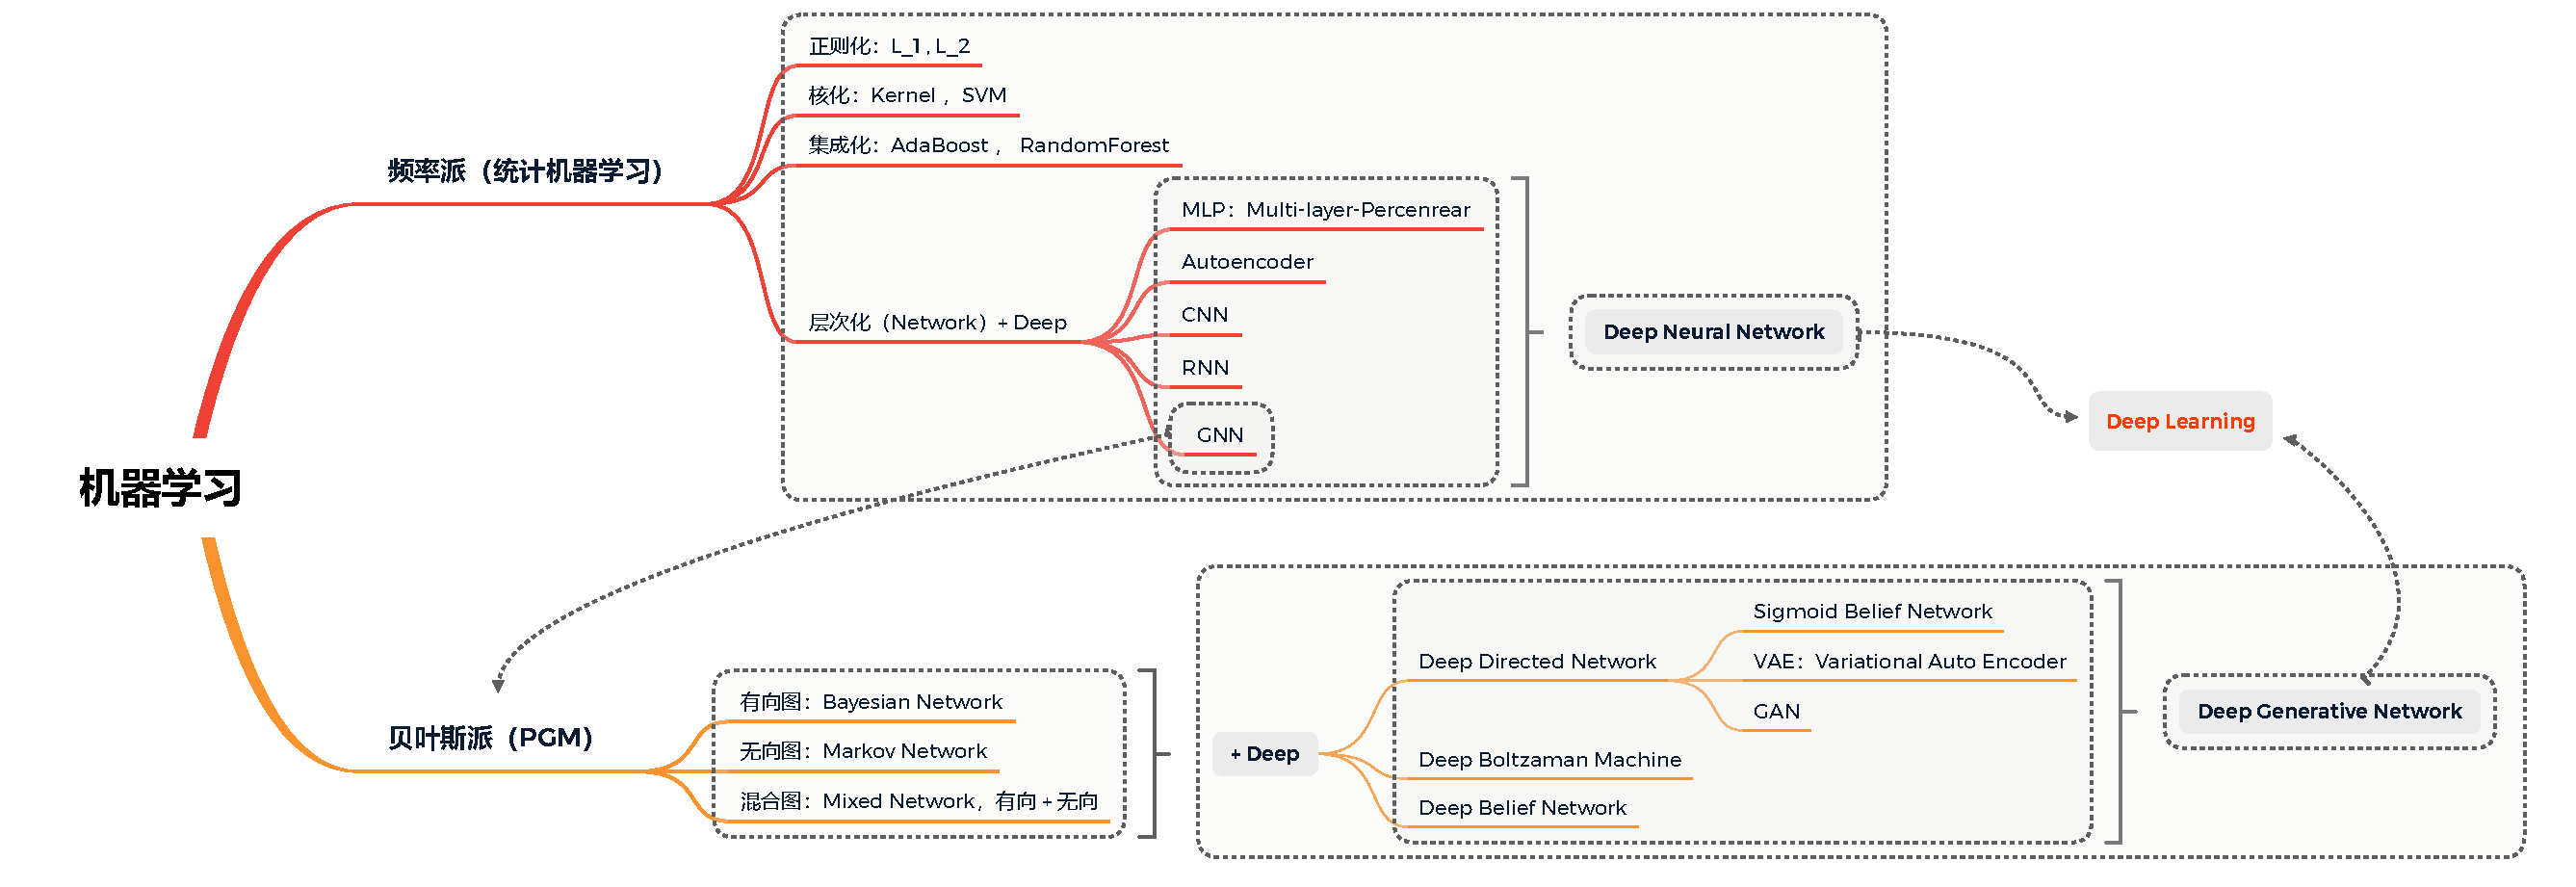
\includegraphics[width=\textwidth]{ML.pdf}
      \end{figure}
    \end{column}
  \end{columns}
\end{frame}

% ---------------------------------------------------------------------------


% ---------------------------------------------------------------------------
\subsection{table}
% ---------------------------------------------------------------------------

% ---------------------------------------------------------------------------
\begin{frame}{数据与tabular环境}
  \begin{table}[H]
    \tiny
    \centering
    %\setlength{\tabcolsep}{-3pt}
    \resizebox{!}{3.0cm}{\begin{tabular}{@{\extracolsep{\fill}}*{3}{l}}
  \toprule
      Category of your contents & Different types of each  Category & other type of  your data \\
      \midrule
      & Different types of each  Category & other type of  your data\\
      & \hrulefill~~ & \hrulefill~~ \\
      & \multicolumn{1}{l}{\dotfill} &  \multicolumn{1}{l}{\dotfill} \\
      & \multicolumn{2}{c}{\hrulefill~~~ $\theta^{-1}$kg ~~~\hrulefill } \\ %\dotfill  $\theta^{-1}$kg ~~~\hrulefill
  \multirow{12}{*}{Type of date (numbers)}
      & 0.0056 $\pm$ 0.0097, 0.0021 $\pm$ 4.0056 & 3.5 $\times$ 10$^{5}$ ; 5.43 (9.30\%) \\
      & 0.0056 $\pm$ 0.0097, 0.0021 $\pm$ 4.0056 & 3.5 $\times$ 10$^{5}$ ; 5.43 (9.30\%) \\
      & 0.0056 $\pm$ 0.0097, 0.0021 $\pm$ 4.0056 & 3.5 $\times$ 10$^{5}$ ; 5.43 (9.30\%) \\
      & 0.0056 $\pm$ 0.0097, 0.0021 $\pm$ 4.0056 & 3.5 $\times$ 10$^{5}$ ; 5.43 (9.30\%) \\
      & 0.0056 $\pm$ 0.0097, 0.0021 $\pm$ 4.0056 & 3.5 $\times$ 10$^{5}$ ; 5.43 (9.30\%) \\
      & 0.0056 $\pm$ 0.0097, 0.0021 $\pm$ 4.0056 & 3.5 $\times$ 10$^{5}$ ; 5.43 (9.30\%) \\
      & 0.0056 $\pm$ 0.0097, 0.0021 $\pm$ 4.0056 & 3.5 $\times$ 10$^{5}$ ; 5.43 (9.30\%) \\
      & 0.0056 $\pm$ 0.0097, 0.0021 $\pm$ 4.0056 & 3.5 $\times$ 10$^{5}$ ; 5.43 (9.30\%) \\
      & 0.0056 $\pm$ 0.0097, 0.0021 $\pm$ 4.0056 & 3.5 $\times$ 10$^{5}$ ; 5.43 (9.30\%) \\
      & 0.0056 $\pm$ 0.0097, 0.0021 $\pm$ 4.0056 & 3.5 $\times$ 10$^{5}$ ; 5.43 (9.30\%) \\
      & 0.0056 $\pm$ 0.0097, 0.0021 $\pm$ 4.0056 & 3.5 $\times$ 10$^{5}$ ; 5.43 (9.30\%) \\
      & 0.0056 $\pm$ 0.0097, 0.0021 $\pm$ 4.0056 & 3.5 $\times$ 10$^{5}$ ; 5.43 (9.30\%) \\
      \hline
  \multirow{3}{*}{Mathematical formulas}
     & $\frac{\mu^2}{\pi-2\theta}\times \sqrt[3]{\|\nu_{i}-\hat{\phi\|}}+\lim\limits_{s\to\infty}\int_{0}^{+\infty}f(x)e^{xsi}{\rm d}x$ & $f(x)\in C^{1}[0,+\infty]$, $\|f(x^{n})\|_{2}\leqslant \lambda$ \\
     &$\frac{\mu^2}{\pi-2\theta}\times \sqrt[3]{\|\nu_{i}-\hat{\phi\|}}+\lim\limits_{s\to\infty}\int_{0}^{+\infty}f(x)e^{xsi}{\rm d}x$ & $f(x)\in C^{1}[0,+\infty]$, $\|f(x^{n})\|_{2}\leqslant \lambda$ \\
     & $\frac{\mu^2}{\pi-2\theta}\times \sqrt[3]{\|\nu_{i}-\hat{\phi\|}}+\lim\limits_{s\to\infty}\int_{0}^{+\infty}f(x)e^{xsi}{\rm d}x$ & $f(x)\in C^{1}[0,+\infty]$, $\|f(x^{n})\|_{2}\leqslant \lambda$ \\
     \hline
  \multirow{7}{*}{Language description}
      & This is the element described in your language & Mathematical language description \\
      & This is the element described in your language & Mathematical language description\\
      & This is the element described in your language & Mathematical language description \\
      & This is the element described in your language & Mathematical language description \\
      & This is the element described in your language & Mathematical language description \\
      & This is the element described in your language & Mathematical language description\\
      & This is the element described in your language & Mathematical language description\\
      \hline
  \multirow{8}{*}{Projection data}
      & 3.5 $\times$ 10$^{5}$ This is the element described in your language&  0.0056 $\pm$ 0.0097, 0.0021 $\pm$ 4.0056 \\
      & 3.5 $\times$ 10$^{5}$ This is the element described in your language&  0.0056 $\pm$ 0.0097, 0.0021 $\pm$ 4.0056 \\
      & 3.5 $\times$ 10$^{5}$ This is the element described in your language&  0.0056 $\pm$ 0.0097, 0.0021 $\pm$ 4.0056 \\
      & 3.5 $\times$ 10$^{5}$ This is the element described in your language&  0.0056 $\pm$ 0.0097, 0.0021 $\pm$ 4.0056 \\
      & 3.5 $\times$ 10$^{5}$ This is the element described in your language&  0.0056 $\pm$ 0.0097, 0.0021 $\pm$ 4.0056 \\
      & 3.5 $\times$ 10$^{5}$ This is the element described in your language&  0.0056 $\pm$ 0.0097, 0.0021 $\pm$ 4.0056\\
      & 3.5 $\times$ 10$^{5}$ This is the element described in your language&  0.0056 $\pm$ 0.0097, 0.0021 $\pm$ 4.0056 \\
      & 3.5 $\times$ 10$^{5}$ This is the element described in your language&  0.0056 $\pm$ 0.0097, 0.0021 $\pm$ 4.0056 \\
      & 3.5 $\times$ 10$^{5}$ This is the element described in your language&  0.0056 $\pm$ 0.0097, 0.0021 $\pm$ 4.0056 \\
  \bottomrule
    \end{tabular}
    }
    \caption{Contents of different types of tables.}
  \end{table}  
  \end{frame}
% ---------------------------------------------------------------------------

% ---------------------------------------------------------------------------
\begin{frame}
  \frametitle{Word2Vec}
  \begin{table}[h]
    \scriptsize
    \setlength{\tabcolsep}{5pt}
    \centering
    \begin{tabular}{|c|c|c|c|c|c|c|c|c|c|c|c|}
      \hline
        \multicolumn{3}{|c|}{topic 1}
      & \multicolumn{3}{c|}{topic 2}
      & \multicolumn{3}{c|}{topic 3}
      & \multicolumn{3}{c|}{topic 4}\\  \hline
     1 & 科技 & 0.9995 & 2 & 板块 & mm    &3&  科技  & mm   & 4 & 3500 & mm \\   
     1 & 板块 & 0.9994 & 2 & 锂电池 & mm  &3&  新能源 & mm  & 4 & 反弹 & mm \\ 
     1 & 调整 & 0.9994 & 2 & a股 & mm     &3&  in & 机构    & 4 & 指数 &  \\  
     1 & 资金 & 0.9994 & 2 & 芯片 & mm    &3&  in & 板块    & 4 & 清仓 &  \\  
     1 & 业绩 & 0.9994 & 2 & 散户 & mm    &3&  in & 半导体   & 4 & 券商 & mm \\  
     1 & 公司 & 0.9994 & 2 & 震荡 & mm    &3&  in & 中国    & 4 & 科技 & mm \\   
     1 & 股价 & 0.9994 & 2 & 早盘& mm     &3&  in & 芯片    & 4 & in & mm \\  
     1 & 股市 & 0.9994 & 2 & inches& mm   &3&  in & mm      & 4 & in & mm \\  
     1 & 大跌 & 0.9994 & 2 & inches& mm   &3&  in & mm      & 4 & in & mm \\  
     1 & 基金 & 0.9994 & 2 & inches& mm   &3&  in & mm      & 4 & in & mm \\ \hline 
    \end{tabular}
    \caption{Word2Vec of texts}
    \label{tab:Margin_settings}
  \end{table}
\end{frame}
% ---------------------------------------------------------------------------

% ---------------------------------------------------------------------------
\section{Other Features}
% ---------------------------------------------------------------------------

% ---------------------------------------------------------------------------
\begin{frame}
  \frametitle{Structural Features}
  \begin{block}{Levels of Structure}
    \begin{itemize}
      \item usual \LaTeX\ \textbackslash{}section, \textbackslash{}subsection commands
      \item `frame' environments provide slides
      \item `block' environments divide slides into logical sections
      \item `columns' environments divide slides vertically (example later)
      \item overlays (\`a la prosper) change content of slides dynamically
    \end{itemize}
  \end{block}
  
  \begin{example}[Overlay Alerts]
    On the first overlay, \alert<1>{this text} is highlighted (or \emph{alerted}).\\ On the second, \alert<2>{this text} is.
  \end{example}
\end{frame}
% ---------------------------------------------------------------------------

% ---------------------------------------------------------------------------
\begin{frame}{Algoritmos 代码1}
  \begin{algorithm}[H]
      \SetAlgoLined
      \LinesNumbered
      \SetKwInOut{Input}{input}
      \SetKwInOut{Output}{output}
      \Input{x: float, y: float}
      \Output{r: float}
      \While{True}{
        r = x + y\;
        \eIf{r >= 30}{
         ``O valor de $r$ é maior ou iqual a 10.''\;
         break\;
         }{
         ``O valor de $r$ = '', r\;
        }
       }
       \caption{Algorithm Example}
  \end{algorithm}
\end{frame}
% ---------------------------------------------------------------------------

% ---------------------------------------------------------------------------
\begin{frame}{Reviewing DeepWalk algorithm}
  \begin{algorithm}[H]
    \caption{Reviewing random walk + skip gram}%算法名字
    \LinesNumbered % 要求显示行号
    % \KwIn{input parameters A, B, C}%输入参数
    % \KwOut{output result}%输出
    % some description\; %\;用于换行
    \For {n = 1 , 2 ,\dots, N} {
         Pick $w_{1}^{n}$ according to a probability distribution $P\left(w_{1}\right)$.
          Generate a vertex sequence $\left(w_{1}^{n}, \cdots, w_{L}^{n}\right)$ of length $L$ by a random walk on network $G$ \;
          \For {j = 1 , 2 ,\dots, L-T} {
            \For {r = 1 , 2 ,\dots, T} {
              Add vertex-context pair $\left(w_{j}^{n}, w_{j+r}^{n}\right)$ to multiset $\mathcal{D}$ \;
              Add vertex-context pair $\left(w_{j+r}^{n}, w_{j}^{n}\right)$ to multiset $\mathcal{D}$
            }
          }
    }
    Run SGNS on $ \mathcal{D}$ with $b$  negative samplpes.
  \end{algorithm}
\end{frame}
% ---------------------------------------------------------------------------

% ---------------------------------------------------------------------------
\begin{frame}[fragile]
  \frametitle{Code blocks}
  % \begin{lstlisting}[language=R]
  % # Say hello in R
  % hello <- function(name) paste("hello", name)
  % \end{lstlisting}

\begin{uncoverenv}<1->
  \begin{lstlisting}[language=Python]
    # Say hello in Python
    def hello(name):
    return("Hello" + " " + name)
  \end{lstlisting}
\end{uncoverenv}
    
\begin{uncoverenv}<2->
  \begin{lstlisting}[language=C]
    /* Say hello in C */
    #include <stdio.h>
    int main()
    {
      char name[256];
      fgets(name, sizeof(name), stdin);
      printf("Hello %s", name);
      return(0);
    }
  \end{lstlisting}
  \end{uncoverenv}
\end{frame}
% ---------------------------------------------------------------------------

% ---------------------------------------------------------------------------
\begin{frame}
  \frametitle{Theorems and Proofs}
  \framesubtitle{The proof uses \textit{reductio ad absurdum}.}
  
  \begin{theorem}
    There is no largest prime number.
  \end{theorem}

  \begin{proof}
    \begin{enumerate}
      \item<1-| alert@1> Suppose $p$ were the largest prime number.
      \item<2-> Let $q$ be the product of the first $p$ numbers.
      \item<3-> Then $q+1$ is not divisible by any of them.
      \item<1-> But $q + 1$ is greater than $1$, thus divisible by some prime
      number not in the first $p$ numbers.\qedhere
    \end{enumerate}
  \end{proof}
  \end{frame}
 % ---------------------------------------------------------------------------

 % ---------------------------------------------------------------------------
  \begin{frame}
    \frametitle{Blocks}
  
    \begin{block}{Normal block}
  A \alert{set} consists of elements.
  \end{block}
  
  \begin{alertblock}{Alert block}
  $2=2$.
  \end{alertblock}
  
  \begin{exampleblock}{Example block}
  The set $\{1,2,3,5\}$ has four elements.
  \end{exampleblock}
  
  \end{frame}
% ---------------------------------------------------------------------------


% \appendix 
\section{\appendixname}


\frame{Details}

% ---------------------------------------------------------------------------
\begin{frame}[allowframebreaks]{参考文献}
  \scriptsize
  \begin{thebibliography}{}
  \setbeamertemplate{bibliography item}[online]
        \bibitem{GK2020}
        Karsten Borgwardt. \ and Elisabetta Ghisu.
        \newblock \emph{Graph Kernels}, 2020.
        \newblock \url{https://arxiv.org/pdf/2011.03854v2.pdf}

  \setbeamertemplate{bibliography item}[triangle]
    \bibitem{AM1969}  
    刘忠雨.\ and 李彦霖. \ and 周洋
    \newblock \emph{深入浅出图神经网络}.
    \newblock 机械工业出版社,2019

  \setbeamertemplate{bibliography item}[article]
    \bibitem{velivckovic2017graph}
    Petar and Cucurull, Guillem and Casanova, Arantxa and Romero, Adriana and Lio, Pietro and Bengio, Yoshua
    \newblock \emph{Graph attention networks}, 2017.
    \newblock \url{https://arxiv.org/pdf/1710.10903.pdf}

    \setbeamertemplate{bibliography item}[article]
    \bibitem{kipf2016semi}
    Kipf, Thomas N and Welling, Max
    \newblock \emph{Semi-supervised classification with graph convolutional networks}, 2016.
    \newblock \url{https://arxiv.org/pdf/1609.02907.pdf?source=post_page---------------------------}

    \setbeamertemplate{bibliography item}[text]
    \bibitem{孙建东zhihu}
    孙建东
    \newblock \emph{《Semi-Supervised Classification with Graph Convolutional Networks》阅读笔记}, 2018,知乎.
    \newblock \url{https://zhuanlan.zhihu.com/p/31067515}

  \end{thebibliography}
\end{frame}
% ---------------------------------------------------------------------------

% ---------------------------------------------------------------------------
\begin{frame}[plain]
  \begin{center}
    {\Huge\calligra Thanks!}
  \end{center}
\end{frame}
% ---------------------------------------------------------------------------

\end{document} 